\documentclass[12pt, a4paper]{article}

\usepackage[slovene, english]{babel}
\usepackage[utf8]{inputenc}
\usepackage{amsmath, amsfonts}
\usepackage{url}
\usepackage{graphicx}
%\usepackage{tikz}
\usepackage{textpos}
\usepackage{wrapfig}
\usepackage{amsthm}
%\usepackage{enumitem}
\usepackage{physics}

\newtheorem{izrek}{Izrek}
\newtheorem{trditev}{Trditev}
\newtheorem{lema}{Lema}
\newtheorem{definicija}{Definicija}
\newtheorem{pos}{Posledica}
\newtheorem{zgled}{Zgled}
\newtheorem{naloga}{Naloga}

\newcommand{\R}{\mathbb R}
\newcommand{\N}{\mathbb N}
\newcommand{\Z}{\mathbb Z}
\newcommand{\C}{\mathbb C}
\newcommand{\Q}{\mathbb Q}

\renewcommand{\mod}{\operatorname{mod}}

\title{Funkcije več spremenljivk}
\author{Karmen Zupančič, Žiga Flajs, Jakob Svetina \\ Mentor: Žan Hafner Petrovski}
\date{
\includegraphics[width = 6cm]{logo_MaRS2017.png}}

\begin{document}
\selectlanguage{slovene}
\maketitle

\begin{abstract}
V članku spoznamo funkcije več spremenljivk in se previdno dotaknemo pomembnih tem iz analize. Začnemo z grafi funkcij dveh spremenljivk, potem pa se osredotočimo na polarne in sferične koordinate, s pomočjo katerih pridemo do sicer že znanih rezultatov, ampak na nov in širše uporaben način. Zaključimo pa s posebno funkcijo, ki predstavlja razširitev fakultete na pozitivna realna števila.
\end{abstract}

\section{Uvod}
Vsak naj bi poznal funkciije ene spremenljivke, saj se jih obravnava že v osnovni šoli. Kdor potem nadaljuje šolanje, se z njimi še bolje spozna, redki pa se spoznajo s funkcijami več spremenljivk. Grafi takih funkcij so dosti težje predstavljivi kot grafi funkcij ene spremenljivke, ki jih lahko dokaj enostavno upodobimo na ravnini. Čim več spremenljivk nastopa v prostoru iz katerega slikamo, tem bolj zapleteni so njihovi grafi, zapletenost pa v tem primeru vodi do večje svobode in nam odpira vrata do bolj abstraktnih idej.

\section{Funkcije dveh spemenljivk}

\begin{definicija}
\textbf{Funkcija dveh neodvisnih spremenljivk} je predpis, ki vsakemu paru $(x,y)$ iz podmnožice ravnine predpiše natančno določeno realno število.
Je preslikava $R^2 \rightarrow R$.
$$f:(x,y) \Rightarrow z=f(x,y)$$

\end{definicija}

Realno število, ki je prirejeno spremenljivkam v trorazsežnem prostoru pomeni višino nad točko. Upodabljamo lahko le funkcije z do tremimi spremenljivkami, za sistem štirih ali večih spemenljivk pa je upodabljanje nemogoče. Za razliko od funkcij z eno spremenljivko upodabljamo funkcije dveh spremenljivk s ploskvijo, ki ima enačbo $u-f(x,y)=0$. Spoznali smo nekaj preprostih funkcij, ogledali pa smo si tudi primere zahtevnejših funkcij dveh spremenljivk.

\begin{zgled}
Funkcija $f(x,y)=x^2+y^2$ Graf funkcije je dvorazsežni objekt v trorazsežnem prostoru.
\end{zgled}

\begin{figure}[h!]
\centering
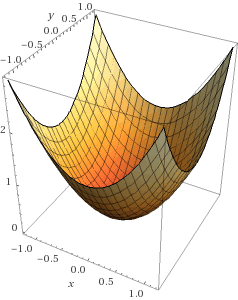
\includegraphics{slika_funkcije.PNG}
\caption{Graf funkcije f(x,y)}
\end{figure}

\newpage
\begin{zgled}
Primer zahtevnejše funkcije $g(x,y)=x^2 sin(x)y^3$ 
\end{zgled}

\begin{figure}[h!]
\centering
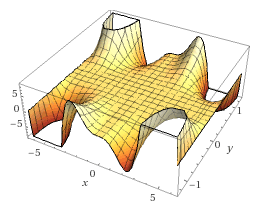
\includegraphics{funkcija_2.PNG}
\caption{Graf funkcije g(x,y)}
\end{figure}

\section{Volumen krogle}

Izračunali smo tudi volumen krogle z različnimi metodami. Začnimo s to, ki smo jo spoznali že v gimnaziji, kasneje pa bomo do iste formule prišli še na drug način. 

\begin{zgled} 
Izračun prostornine vrtenine, ki nastane z vrtenjem funkcije $f(x)=\sqrt{(1-x^2)}$ .

$$V=\pi \int_{a}^b{f(x)}^2dx$$
$$V=\pi \int_{-1}^1{{\sqrt{(1-x^2)}}}^2dx=\pi(x-\frac{x^3}{3})\mid_{-1}^1= \pi (1-\frac{1}{3})-\pi (-1+\frac{1}{3})$$
$$V=\frac{4}{3}\pi$$
\end{zgled}


\section{Izrek o zamenjavi spremenljivk v integralu}
Najprej se bomo seznanili s primerom zamenjave ene spremenljivke potem pa bomo spoznali še zamenjavo dveh in treh spremenljivk v integralu.
\\
Naj bo $f$ zvezna na $[a,b]$ in $\phi$ zvezno odvedljiva funkcija, ki interval $[\alpha,\beta]$ preslika bijektivno na interval $[a,b]$ tako, da je  $\phi(\alpha)=a$ in $\phi(\beta)=b$. Tedaj je

$$\int_{a}^bf(x)\mathrm{d} x=\int_{\alpha}^{\beta}f(\phi(t))\phi'(t)\mathrm{d} t$$

Na podoben način lahko zamenjamo več spremenljivk. 
\begin{izrek}
Naj bo $U \subset \mathbb{R}^n$ odprta množica z volumnom $\neq 0$ in $g:U \rightarrow \mathbb{R}^n$ dovolj lepa preslikava. Naj bo $\big | \det Dg(t) \big |\neq 0$ za vse $t \in U$ in omejena na $U$. Predpostavimo, da ima $g(U)$ volumen. Za vsako integrabilno funkcijo $f:g(U) \rightarrow \mathbb{R}$ velja:

$$\int_{g(U)}^{}f(x) \mathrm{d} V=\int_{U}^{}f(g(t)) \big |\det Dg(t) \big | \mathrm{d} V$$
\end{izrek}

%%%%%%%%%%%%%%%%%%%%%%%%%%%%%%%%%%%%%%
\section{Računanje determinante reda 2 in 3}

Poglejmo si kako se računa determinanta reda 2 in 3. Tukaj so eksplicitne formule za njihov izračun.

\[
\begin{vmatrix}
    a& b  \\
   c &d \\
\end{vmatrix}
=ad-bc
\]

\[
\begin{vmatrix}
 a&b&c\\
 d&e&f\\
 g&h&i\\
\end{vmatrix}
=a\begin{vmatrix}
e&f\\
h&i\\
\end{vmatrix}-b\begin{vmatrix}
d&f\\
g&i\\
\end{vmatrix}+c\begin{vmatrix}
d&e\\
g&h\\
\end{vmatrix}
\]



%%%%%%%%%%%%%%%%%%%%%%%%%%%%%%%%%%%%%%

\section{Polarne koordinate}
Polarni koordinatni sistem je ravninski koordinatni sistem, ki je osnova za sferični koordinatni sistem. Točko v polarnem koordinatnem sistemu podamo z dvema polarnima koordinatama:
\begin{itemize}
\item $r$ - razdalja od točke do koordinatnega izhodišča (dolžina vektorja $\vec{r}$)
\item $\phi$ - kot med $x$-osjo in smerjo vektorja $\vec{r}$
\end{itemize}

Da iz polarnih koordinat dobimo koordinati kartezičnega koordinatnega sistema $x$ in $y$, uporabimo preslikavo $g:[ 0,\infty)    [0,2\pi]  \rightarrow  \mathbb{R}^2$ s sledečim predpisom:
$$g(r,\phi) = (r \cos \phi, r \sin \phi)$$

Kartezični koordinati torej z $r$ in $\phi$ izrazimo takole:
\begin{itemize}
\item $x=r \cos \phi$
\item $y=r \sin \phi$
\end{itemize}

\begin{figure}[h!]
\centering
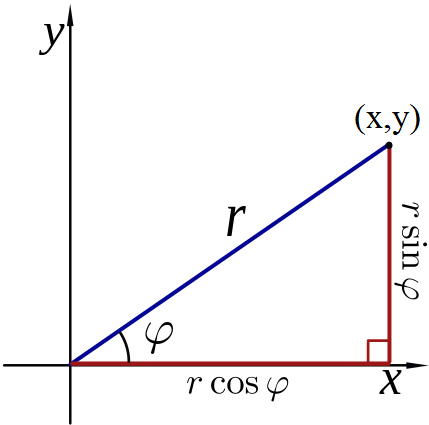
\includegraphics[width=.4\textwidth]{polarne_koordinate.png}
\end{figure}



\section{Sferične koordinate}

Sferični ali krogelni koordinatni sistem je krivočrtni sistem koordinat v trirazsežnem prostoru, s pomočjo katerega enolično določimo lego točk na sferi ali sferoidu. Za določanje lege točke v prostoru vedno potrebujemo tri koordinate. Pri sfernem koordinatnem sistemu uporabljamo sferične koordinate:
\begin{itemize}
\item $r$ - razdalja od točke do koordinatnega izhodišča (dolžina vektorja $\vec{r}$)
\item $\phi$ - kot med $x$-osjo in smerjo pravokotne projekcije vektorja $\vec{r}$ na ravnino $x$-$y$
\item $\theta$ - kot med ravnino $x$-$y$ in vektorjem $\vec{r}$
\end{itemize}

Da iz polarnih koordinat dobimo koordinate kartezičnega koordinatnega sistema $x$, $y$ in $z$, uporabimo preslikavo $g:  [ 0,\infty)    [0,2\pi]    [-\frac{\pi}{2}]  \rightarrow \mathbb{R}^3 $ s predpisom:
$$g(r,\phi, \theta) = (r \cos \phi \cos \theta, r \sin \phi \cos \theta, r \sin \theta)$$

Dobimo koordinate:
\begin{itemize}
\item $x=r \sin \phi \cos \theta$
\item $y=r \cos \phi  \cos \theta $
\item $z=r \sin \theta$
\end{itemize}




\section{Parcialni odvod}

%parcialne odvode moramo spoznati, da lahko uporabimo zgornji izrek

Denimo, da je $f : \mathbb{R}^2 \rightarrow \mathbb{R} $ je funkcija dveh spremenljivk.

Parcialna odvoda po $x$ in po $y$ funkcije $f$ v točki $(a, b)$ definiramo (podobno kot odvod pri funkciji ene spremenljivke) kot limiti ustreznih parcialnih diferenčnih kvocientov (pri pogoju, da ti dve limiti obstajata):
$$
f_x(a, b)= \frac{\partial f}{\partial x}(a, b) = \lim_{h\to\infty} \frac{f(a+h, b)}{h}
$$
$$
f_y(a, b)= \frac{\partial f}{\partial y}(a, b) = \lim_{k\to\infty} \frac{f(a, b+k)}{k}
$$

Parcialna odvoda torej izračunamo tako, da odvajamo funkcijo na $x$ oziroma na $y$ po znanih pravilih za odvajanje funkcij ene spremenljivke, pri čemer smatramo drugo spremenljivko za konstanto.

\begin{zgled}

Za funkcijo $f(x, y)= x^2+xy+y^2$ je $\frac{\partial f}{\partial x}= 2x+y+y^2$ in $\frac{\partial f}{\partial y}= 2y+x+x^2$.

\end{zgled}

\section{Jacobijeva matrika}
Jacobijeva matrika je matrika, ki jo sestavljajo parcialni odvodi prvega reda.
Matrika reda 2 ima obliko:
$$
Jg(x_1,x_2)=
\begin{bmatrix}
\frac{\partial g_1}{\partial x_1} & \frac{\partial g_2}{\partial x_1}  \\
\frac{\partial g_1}{\partial x_2} & \frac{\partial _2}{\partial x_2} 
\end{bmatrix}
$$

\noindent Matrika reda 3 ima obliko:
$$
Jg(x_1,x_2,x_3)=
\begin{bmatrix}
\frac{\partial g_1}{\partial x_1}  & \frac{\partial g_2}{\partial x_1}  & \frac{\partial g_3}{\partial x_1}  \\
\frac{\partial g_1}{\partial x_2}  & \frac{\partial g_2}{\partial x_2}  & \frac{\partial g_3}{\partial x_2}  \\
\frac{\partial g_1}{\partial x_3}  & \frac{\partial g_2}{\partial x_3}  & \frac{\partial g_3}{\partial x_3} 
\end{bmatrix}
$$



\section{Ploščina kroga in volumen krogle}

\begin{naloga}
S pomočjo polarnih koordinat in parcialnih odvodov izračunaj formulo za računanje ploščine kroga. \\
\emph
{Najprej izračunamo parcialne odvode polarnih koordinat:}

\begin{itemize}
\item $\frac{\partial x}{\partial r}= \cos \phi$
\item $\frac{\partial x}{\partial \phi}= r  (-\sin \phi)$
\item $\frac{\partial y}{\partial r}= \sin \phi$
\item $\frac{\partial y}{\partial \phi}= r  \cos \phi$ \\
\end{itemize}
\emph
{Parcialni odvod izračunamo, da lahko izračunamo Jacobijevo determinanto s pomočjo Jacobijeve matrike:}
\\
\begin{center}
 {
$\det (Jg)(r,\phi)=$ \large $ \begin{vmatrix} \frac{\partial x}{\partial r}  &  \frac{\partial x}{\partial \phi}  \\  \frac{\partial y}{\partial r}  &  \frac{\partial y}{\partial \phi}  \end{vmatrix} $ $=$ \normalsize $\begin{vmatrix} \cos \phi & -r \sin \phi \\ \sin \phi & r \cos \phi \end{vmatrix} $  $= r$
}
\end{center}

\emph
{Dobimo determinanto diferenciala preslikave $g$, ki jo vstavimo v dvojni integral:} \\

$ \int^{2\pi}_{0} \int^{R}_{0}   \begin{vmatrix} \det Dg \end{vmatrix}  \mathrm{d} r \mathrm{d}\phi \\
 =  \int^{2\pi}_{0} \int^{R}_{0}  r \mathrm{d} r \mathrm{d}\phi \\
 =  \int^{2\pi}_{0} \frac{r^2}{2} \big|^{R}_{0} \mathrm{d}\phi \\
 =  \int^{2\pi}_{0} \frac{R^2}{2} \mathrm{d}\phi \\
 =  \frac{R^2}{2} \phi  \big|^{2\pi}_{0} \\
 =  \frac{R^2}{2} 2\pi \\
 =  \pi R^2 $ \\

\emph
{Ugotovimo, da smo dobili formulo za računanje površine kroga:}
$$
S=\pi r^2
$$
\end{naloga}


\begin{naloga}
S pomočjo sferičnih koordinat in parcialnih odvodov izračunaj formulo za volumen krogle.

\emph{Podobno kot prej izračunamo parcialne odvode in jih vpišemo v matriko, s katero izračunamo determinanto:}
\\
\begin{center}
$ \det (Jg)(r,\phi, \theta)$ $=$  \\ $=$ \large  $\begin{vmatrix} \frac{\partial x}{\partial r}  &  \frac{\partial x}{\partial \phi} &  \frac{\partial x}{\partial z} \\  \frac{\partial y}{\partial r}  &  \frac{\partial y}{\partial \phi} &  \frac{\partial x}{\partial z} \\ \frac{\partial \theta}{\partial r}  &  \frac{\partial \theta}{\partial \phi} &  \frac{\partial \theta}{\partial z} \end{vmatrix} $ 
$=$  \normalsize $ \begin{vmatrix} \cos \phi  \cos \theta & \sin \phi  \cos \theta & \sin \theta \\ r \sin \phi  \cos \theta  & r \cos \phi  \cos \theta  & 0 \\ r \cos \phi  (-\sin \theta)  & r \sin \phi  (-\sin \theta)  & r \cos \theta \\ \end{vmatrix} $  $=$ $r^2 \cos \theta $
\end{center}

\emph{Determinanto vstavimo v trojni integral:} \\

$ \int^{\frac {\pi}{2}}_{- \frac {\pi}{2}} \int^{2\pi}_{0} \int^{R}_{0}  \big | \det Dg \big | \mathrm{d} r \mathrm{d}\phi \mathrm{d}\theta  \\
 =  \int^{\frac {\pi}{2}}_{- \frac {\pi}{2}} \int^{2\pi}_{0} \int^{R}_{0}   r^2 \cos \theta   \mathrm{d} r \mathrm{d}\phi \mathrm{d}\theta  \\
 =  \int^{\frac {\pi}{2}}_{- \frac {\pi}{2}} \int^{2\pi}_{0} \cos \theta \frac {r^3}{3} \big |^{R}_{0} \mathrm{d}\phi \mathrm{d}\theta  \\
 =  \int^{\frac {\pi}{2}}_{- \frac {\pi}{2}} \int^{2\pi}_{0} \cos \theta \frac {R^3}{3} \mathrm{d}\phi \mathrm{d}\theta  \\
 =  \int^{\frac {\pi}{2}}_{- \frac {\pi}{2}} \cos \theta \frac {R^3}{3} \big |^{2 \pi}_{0} \mathrm{d} \theta  \\
 =  \int^{\frac {\pi}{2}}_{- \frac {\pi}{2}} \frac {2 \pi R^3}{3} \cos \theta \mathrm{d} \theta  \\
 =  \frac {2 \pi R^3}{3} \sin \theta \big |^{\frac {\pi}{2}}_{-\frac {\pi}{2}}  \\
 =  (2) \frac {2 \pi R^3}{3}  \\
 =  \frac {4 \pi R^3}{3} $ \\

\emph
{Ugotovimo, da smo dobili formulo za računanje volumna krogle:}
$$
V=\frac{4\pi r^3}{3}
$$
\end{naloga}








%http://www.fmf.uni-lj.si/~hladnik/Analiza/ParcialniOdvodi.pdf














\end{document}